\section{Auswertung}
\subsection{Bestimmung der Schwingungsdauer}
Trägt man für die beiden Messungen ($\alpha=\SI{\pm45}{\degree}$) die Auslenkung gegen die Zeit auf, ergeben sich folgende Darstellungen:
\begin{figure}[!htbp]
\centering
   % GNUPLOT: LaTeX picture with Postscript
\begingroup
  \makeatletter
  \providecommand\color[2][]{%
    \GenericError{(gnuplot) \space\space\space\@spaces}{%
      Package color not loaded in conjunction with
      terminal option `colourtext'%
    }{See the gnuplot documentation for explanation.%
    }{Either use 'blacktext' in gnuplot or load the package
      color.sty in LaTeX.}%
    \renewcommand\color[2][]{}%
  }%
  \providecommand\includegraphics[2][]{%
    \GenericError{(gnuplot) \space\space\space\@spaces}{%
      Package graphicx or graphics not loaded%
    }{See the gnuplot documentation for explanation.%
    }{The gnuplot epslatex terminal needs graphicx.sty or graphics.sty.}%
    \renewcommand\includegraphics[2][]{}%
  }%
  \providecommand\rotatebox[2]{#2}%
  \@ifundefined{ifGPcolor}{%
    \newif\ifGPcolor
    \GPcolortrue
  }{}%
  \@ifundefined{ifGPblacktext}{%
    \newif\ifGPblacktext
    \GPblacktexttrue
  }{}%
  % define a \g@addto@macro without @ in the name:
  \let\gplgaddtomacro\g@addto@macro
  % define empty templates for all commands taking text:
  \gdef\gplbacktext{}%
  \gdef\gplfronttext{}%
  \makeatother
  \ifGPblacktext
    % no textcolor at all
    \def\colorrgb#1{}%
    \def\colorgray#1{}%
  \else
    % gray or color?
    \ifGPcolor
      \def\colorrgb#1{\color[rgb]{#1}}%
      \def\colorgray#1{\color[gray]{#1}}%
      \expandafter\def\csname LTw\endcsname{\color{white}}%
      \expandafter\def\csname LTb\endcsname{\color{black}}%
      \expandafter\def\csname LTa\endcsname{\color{black}}%
      \expandafter\def\csname LT0\endcsname{\color[rgb]{1,0,0}}%
      \expandafter\def\csname LT1\endcsname{\color[rgb]{0,1,0}}%
      \expandafter\def\csname LT2\endcsname{\color[rgb]{0,0,1}}%
      \expandafter\def\csname LT3\endcsname{\color[rgb]{1,0,1}}%
      \expandafter\def\csname LT4\endcsname{\color[rgb]{0,1,1}}%
      \expandafter\def\csname LT5\endcsname{\color[rgb]{1,1,0}}%
      \expandafter\def\csname LT6\endcsname{\color[rgb]{0,0,0}}%
      \expandafter\def\csname LT7\endcsname{\color[rgb]{1,0.3,0}}%
      \expandafter\def\csname LT8\endcsname{\color[rgb]{0.5,0.5,0.5}}%
    \else
      % gray
      \def\colorrgb#1{\color{black}}%
      \def\colorgray#1{\color[gray]{#1}}%
      \expandafter\def\csname LTw\endcsname{\color{white}}%
      \expandafter\def\csname LTb\endcsname{\color{black}}%
      \expandafter\def\csname LTa\endcsname{\color{black}}%
      \expandafter\def\csname LT0\endcsname{\color{black}}%
      \expandafter\def\csname LT1\endcsname{\color{black}}%
      \expandafter\def\csname LT2\endcsname{\color{black}}%
      \expandafter\def\csname LT3\endcsname{\color{black}}%
      \expandafter\def\csname LT4\endcsname{\color{black}}%
      \expandafter\def\csname LT5\endcsname{\color{black}}%
      \expandafter\def\csname LT6\endcsname{\color{black}}%
      \expandafter\def\csname LT7\endcsname{\color{black}}%
      \expandafter\def\csname LT8\endcsname{\color{black}}%
    \fi
  \fi
  \setlength{\unitlength}{0.0500bp}%
  \begin{picture}(7200.00,5040.00)%
    \gplgaddtomacro\gplbacktext{%
      \csname LTb\endcsname%
      \put(1078,704){\makebox(0,0)[r]{\strut{} 1.35}}%
      \put(1078,1317){\makebox(0,0)[r]{\strut{} 1.4}}%
      \put(1078,1929){\makebox(0,0)[r]{\strut{} 1.45}}%
      \put(1078,2542){\makebox(0,0)[r]{\strut{} 1.5}}%
      \put(1078,3154){\makebox(0,0)[r]{\strut{} 1.55}}%
      \put(1078,3767){\makebox(0,0)[r]{\strut{} 1.6}}%
      \put(1078,4379){\makebox(0,0)[r]{\strut{} 1.65}}%
      \put(1210,484){\makebox(0,0){\strut{} 0}}%
      \put(2009,484){\makebox(0,0){\strut{} 500}}%
      \put(2808,484){\makebox(0,0){\strut{} 1000}}%
      \put(3607,484){\makebox(0,0){\strut{} 1500}}%
      \put(4406,484){\makebox(0,0){\strut{} 2000}}%
      \put(5205,484){\makebox(0,0){\strut{} 2500}}%
      \put(6004,484){\makebox(0,0){\strut{} 3000}}%
      \put(6803,484){\makebox(0,0){\strut{} 3500}}%
      \put(176,2541){\rotatebox{-270}{\makebox(0,0){\strut{}$y(t) [m]$}}}%
      \put(4006,154){\makebox(0,0){\strut{}$t [s]$}}%
      \put(4006,4709){\makebox(0,0){\strut{}Messung 1}}%
    }%
    \gplgaddtomacro\gplfronttext{%
    }%
    \gplbacktext
    \put(0,0){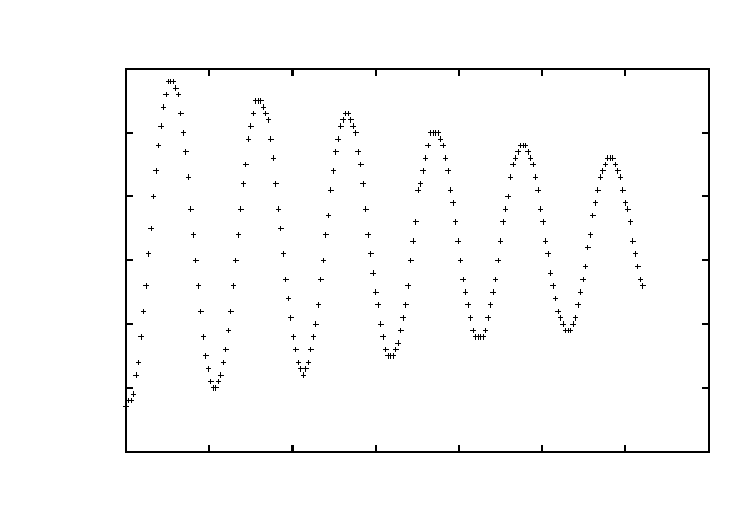
\includegraphics{y-t_1}}%
    \gplfronttext
  \end{picture}%
\endgroup

   \caption{\small{Zeitlicher Verlauf der Auslenkung des Laserstrahls (Messung 1)}}
   \label{img:1}
\end{figure}
\begin{figure}[!htbp]
\centering
   % GNUPLOT: LaTeX picture with Postscript
\begingroup
  \makeatletter
  \providecommand\color[2][]{%
    \GenericError{(gnuplot) \space\space\space\@spaces}{%
      Package color not loaded in conjunction with
      terminal option `colourtext'%
    }{See the gnuplot documentation for explanation.%
    }{Either use 'blacktext' in gnuplot or load the package
      color.sty in LaTeX.}%
    \renewcommand\color[2][]{}%
  }%
  \providecommand\includegraphics[2][]{%
    \GenericError{(gnuplot) \space\space\space\@spaces}{%
      Package graphicx or graphics not loaded%
    }{See the gnuplot documentation for explanation.%
    }{The gnuplot epslatex terminal needs graphicx.sty or graphics.sty.}%
    \renewcommand\includegraphics[2][]{}%
  }%
  \providecommand\rotatebox[2]{#2}%
  \@ifundefined{ifGPcolor}{%
    \newif\ifGPcolor
    \GPcolortrue
  }{}%
  \@ifundefined{ifGPblacktext}{%
    \newif\ifGPblacktext
    \GPblacktexttrue
  }{}%
  % define a \g@addto@macro without @ in the name:
  \let\gplgaddtomacro\g@addto@macro
  % define empty templates for all commands taking text:
  \gdef\gplbacktext{}%
  \gdef\gplfronttext{}%
  \makeatother
  \ifGPblacktext
    % no textcolor at all
    \def\colorrgb#1{}%
    \def\colorgray#1{}%
  \else
    % gray or color?
    \ifGPcolor
      \def\colorrgb#1{\color[rgb]{#1}}%
      \def\colorgray#1{\color[gray]{#1}}%
      \expandafter\def\csname LTw\endcsname{\color{white}}%
      \expandafter\def\csname LTb\endcsname{\color{black}}%
      \expandafter\def\csname LTa\endcsname{\color{black}}%
      \expandafter\def\csname LT0\endcsname{\color[rgb]{1,0,0}}%
      \expandafter\def\csname LT1\endcsname{\color[rgb]{0,1,0}}%
      \expandafter\def\csname LT2\endcsname{\color[rgb]{0,0,1}}%
      \expandafter\def\csname LT3\endcsname{\color[rgb]{1,0,1}}%
      \expandafter\def\csname LT4\endcsname{\color[rgb]{0,1,1}}%
      \expandafter\def\csname LT5\endcsname{\color[rgb]{1,1,0}}%
      \expandafter\def\csname LT6\endcsname{\color[rgb]{0,0,0}}%
      \expandafter\def\csname LT7\endcsname{\color[rgb]{1,0.3,0}}%
      \expandafter\def\csname LT8\endcsname{\color[rgb]{0.5,0.5,0.5}}%
    \else
      % gray
      \def\colorrgb#1{\color{black}}%
      \def\colorgray#1{\color[gray]{#1}}%
      \expandafter\def\csname LTw\endcsname{\color{white}}%
      \expandafter\def\csname LTb\endcsname{\color{black}}%
      \expandafter\def\csname LTa\endcsname{\color{black}}%
      \expandafter\def\csname LT0\endcsname{\color{black}}%
      \expandafter\def\csname LT1\endcsname{\color{black}}%
      \expandafter\def\csname LT2\endcsname{\color{black}}%
      \expandafter\def\csname LT3\endcsname{\color{black}}%
      \expandafter\def\csname LT4\endcsname{\color{black}}%
      \expandafter\def\csname LT5\endcsname{\color{black}}%
      \expandafter\def\csname LT6\endcsname{\color{black}}%
      \expandafter\def\csname LT7\endcsname{\color{black}}%
      \expandafter\def\csname LT8\endcsname{\color{black}}%
    \fi
  \fi
  \setlength{\unitlength}{0.0500bp}%
  \begin{picture}(7200.00,5040.00)%
    \gplgaddtomacro\gplbacktext{%
      \csname LTb\endcsname%
      \put(1078,704){\makebox(0,0)[r]{\strut{} 1}}%
      \put(1078,1038){\makebox(0,0)[r]{\strut{} 1.05}}%
      \put(1078,1372){\makebox(0,0)[r]{\strut{} 1.1}}%
      \put(1078,1706){\makebox(0,0)[r]{\strut{} 1.15}}%
      \put(1078,2040){\makebox(0,0)[r]{\strut{} 1.2}}%
      \put(1078,2374){\makebox(0,0)[r]{\strut{} 1.25}}%
      \put(1078,2709){\makebox(0,0)[r]{\strut{} 1.3}}%
      \put(1078,3043){\makebox(0,0)[r]{\strut{} 1.35}}%
      \put(1078,3377){\makebox(0,0)[r]{\strut{} 1.4}}%
      \put(1078,3711){\makebox(0,0)[r]{\strut{} 1.45}}%
      \put(1078,4045){\makebox(0,0)[r]{\strut{} 1.5}}%
      \put(1078,4379){\makebox(0,0)[r]{\strut{} 1.55}}%
      \put(1210,484){\makebox(0,0){\strut{} 0}}%
      \put(2009,484){\makebox(0,0){\strut{} 500}}%
      \put(2808,484){\makebox(0,0){\strut{} 1000}}%
      \put(3607,484){\makebox(0,0){\strut{} 1500}}%
      \put(4406,484){\makebox(0,0){\strut{} 2000}}%
      \put(5205,484){\makebox(0,0){\strut{} 2500}}%
      \put(6004,484){\makebox(0,0){\strut{} 3000}}%
      \put(6803,484){\makebox(0,0){\strut{} 3500}}%
      \put(176,2541){\rotatebox{-270}{\makebox(0,0){\strut{}$y(t) [m]$}}}%
      \put(4006,154){\makebox(0,0){\strut{}$t [s]$}}%
      \put(4006,4709){\makebox(0,0){\strut{}Messung 2}}%
    }%
    \gplgaddtomacro\gplfronttext{%
    }%
    \gplbacktext
    \put(0,0){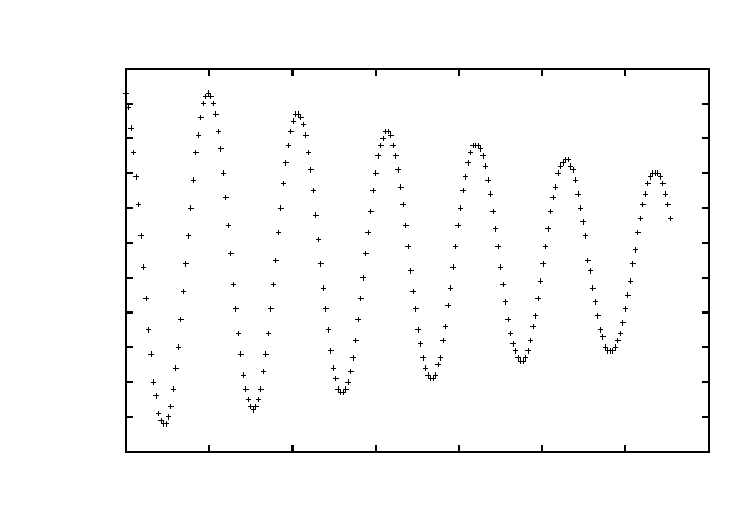
\includegraphics{y-t_2}}%
    \gplfronttext
  \end{picture}%
\endgroup

   \caption{\small{Zeitlicher Verlauf der Auslenkung des Laserstrahls (Messung 2)}}
   \label{img:2}
\end{figure}
\newpage
Hieraus wird zunächst die Ruhelage der Schwingung (Endeinstellung $\bar{y}$) bestimmt (Tab. \ref{tab:1}). Dazu wird über je drei Extrema nach der Beziehung
\begin{align}
\bar{y}_i=\frac{y_i+y_{i+2}+2y_{i+1}}{4}
\end{align}
ein Wert berechnet und anschließend über alle Werte gemittelt. Aus der Fehlerfortpflanzung ergibt sich
\begin{align}
\sigma_{\bar{y}_i}=\frac{\sigma_y}{\sqrt{2}}\\
\Delta_{\bar{y}}=\frac{\sigma_{\bar{y}_i}}{\sqrt{n}}
\end{align}
wobei n die Anzahl der erhaltenen $\bar{y}_i$ ist und $\sigma_y=\SI{0,005}{\meter}$ für alle Messwerte gilt.\\
\ \\
Die Nulllage ($\alpha=\SI{0}{\degree}$) ist der gewichtete Mittelwert der beiden Endeinstellungen
\begin{align}
\bar{y}_0=\frac{\frac{\bar{y}_1}{{\sigma_{\bar{y}_1}}^2}+\frac{\bar{y}_2}{{\sigma_{\bar{y}_2}}^2}}{\frac{1}{{\sigma_{\bar{y}_1}}^2}+\frac{1}{{\sigma_{\bar{y}_2}}^2}}
\end{align}
mit dem Fehler
\begin{align}
\sigma_{\bar{y}_0}=\sqrt{\frac{1}{\frac{1}{{\sigma_{\bar{y}_1}}^2}+\frac{1}{{\sigma_{\bar{y}_2}}^2}}}
\end{align}
Aus der Differenz der Nulldurchgängen lässt sich die Periodendauer bestimmen. Für die Nullstellen ist der Fehler der mittlere quadratische Fehler der beiden direkt neben der Nullstelle liegenden Messwerte.
\begin{align}
\Delta_{t_n}=\sqrt{\left(t_1-\bar{t}\right)^2+\left(t_2-\bar{t}\right)^2}
\end{align}
Aus der Fehlerfortpflanzung ergibt sich der Fehler der einzelnen Bestwerte für die Periodendauer:
\begin{align}
\sigma_{T_n}=\sqrt{2}\Delta_{t_n}
\end{align}
Der Fehler des Mittelwertes ist
\begin{align}
\Delta_T=\frac{\sigma_T}{\sqrt{N}}
\end{align}
Aus den Messwerten berechnet man
\begin{align}
T=\SI{531\pm4}{\second}
\end{align}
\subsection{Berechnung der mittleren Auslenkung und des Auslenkungswinkels}
Nach der Bestimmung der Endeinstellungen und der Nulllage lässt sich für beide Messungen die mittlere Auslenkung $\bar{A}_i$ als Differenz der Endeinstellung zur Nulllage berechnen. Der gewichtete Mittelwert der mittleren Auslenkung y ist also
\begin{align}
y=\frac{\frac{\bar{A}_1}{{\sigma_{\bar{A}_1}}^2}+\frac{\bar{A}_2}{{\sigma_{\bar{A}_2}}^2}}{\frac{1}{{\sigma_{\bar{A}_1}}^2}+\frac{1}{{\sigma_{\bar{A}_2}}^2}}
\end{align} 
mit
\begin{align}
\sigma_{\bar{A}_i}=\sqrt{{\Delta_{\bar{y}_i}}^2+{\sigma_{\bar{y}_0}}^2}\\
\Delta_y=\sqrt{\frac{1}{\frac{1}{{\sigma_{\bar{A}_1}}^2}+\frac{1}{{\sigma_{\bar{A}_2}}^2}}}
\end{align}
Der Auslenkungswinkel $\varphi$ ergibt sich mit
\begin{align}
\varphi=\frac{1}{2}\arctan\left(\frac{y}{l}\right)\\
\sigma_\varphi=\frac{{\sigma_y}^2l^2+{\sigma_l}^2+y^2}{2(y^2+l^2)}
\end{align}
aus der Geometrie des Aufbaus. $l$ ist die Lichtzeigerlänge und durch den Versuchsaufbau vorgegeben (für Wert und Fehlerschätzung vgl. Tab. \ref{tab:2}).
\subsection{Berechnung der Gravitationskonstante}
Für die Berechnung der Gravitationskonstante werden noch weitere Parameter benötigt, welche durch den Versuchsaufbau vorgegeben sind. In Tabelle \ref{tab:2} sind die Werte aufgetragen.
\begin{table}[!htpb]
\begin{tabular}{|l|r|}
\hline 
Lichtzeigerlänge $l$ & \SI{0,265\pm0,0005}{\meter} \\ 
\hline 
Masse der großen Kugeln M & \SI{10,142\pm0,0005}{\kilogram} \\ 
\hline 
Masse der kleinen Kugeln m & \SI{0,002\pm0,0005}{\kilogram} \\ 
\hline 
Radius der kleinen Kugeln r & \SI{0,0075\pm0,00005}{\meter} \\ 
\hline 
Abstand Schwerpunkt-Drehachse der kleinen Kugeln a & \SI{0,024\pm0,0005}{\meter} \\ 
\hline
Abstand Schwerpunkt-Drehachse der großen Kugeln b & \SI{0,1015\pm0,00005}{\meter} \\ 
\hline 
\end{tabular}
\caption{Parameter der Gravitationswaage. Als Fehler wird jeweils die Hälfte des kleinsten angegebenen Skalenteils angenommen.}
\label{tab:2}
\end{table}
\newpage
Zusätzlich wird die Auslenkung $\alpha=\SI{45\pm1}{\degree}$ benötigt. Damit sind alle nötigen Werte vorhanden, um mit der Formel
\begin{align}
\gamma=4\pi^2\varphi\cdot\frac{\left(a^2+b^2-2ab\cos\alpha\right)^{3/2}\cdot\left(a^2+\frac{2}{5}r^2\right)}{abM{\sin\alpha\cdot{T}^2}}
\end{align}
die Gravitationskonstante $\gamma$ zu bestimmen. Der Fehler wird mit der Fehlerfortpflanzung bestimmt:
\begin{align}
\sigma_\gamma=\sqrt{\left(\frac{\partial\gamma}{\partial\varphi}\right)^2{\sigma_\varphi}^2+\left(\frac{\partial\gamma}{\partial{a}}\right)^2{\sigma_a}^2+\left(\frac{\partial\gamma}{\partial{b}}\right)^2{\sigma_b}^2+\left(\frac{\partial\gamma}{\partial\alpha}\right)^2{\sigma_\alpha}^2+\left(\frac{\partial\gamma}{\partial{r}}\right)^2{\sigma_r}^2+\left(\frac{\partial\gamma}{\partial{M}}\right)^2{\sigma_M}^2+\left(\frac{\partial\gamma}{\partial{T}}\right)^2{\sigma_T}^2}
\end{align}
mit
%\begin{align}
%\left(\frac{\partial\gamma}{\partial\varphi}\right)^2=\frac{16\pi^4\left(a^2+\frac{2r^2}{5}\right)^2\cdot\csc^2(\alpha)\cdot(a^2-2ab\cos(\alpha)+b^2)^3}{a^2b^2M^2T^4}\\
%\left(\frac{\partial\gamma}{\partial{a}}\right)^2=\left(-\frac{4\pi^2\varphi\left(a^2+\frac{2r^2}{5}\right)\csc(\alpha)(a^2-2ab\cos(\alpha)+b^2)^{\frac{3}{2}}}{a^2bMT^2}+
%\frac{6\pi^2\varphi\left(a^2+\frac{2r^2}{5}\right)\csc(\alpha)\cdot(2a-2b\cos(\alpha))\cdot\sqrt{a^2-2ab\cos(\alpha)+b^2}}{abMT^2}+
%\frac{8\pi^2\varphi\csc(\alpha)(a^2-2ab\cos(\alpha)+b^2)^{\frac{3}{2}}}{bMT^2}\right)^2\\
%\left(\frac{\partial\gamma}{\partial{b}}\right)^2=\left(\frac{6\pi^2\varphi\left(a^2+\frac{2r^2}{5}\right)\csc(\alpha)\cdot(2-2a\cos(\alpha))\cdot\sqrt{a^2-2ab\cos(\alpha)+b^2}}{abMT^2}-
%\frac{4\pi^2\varphi\left(a^2+\frac{2r^2}{5}\right)\csc(\alpha)(a^2-2ab\cos(\alpha)+b^2)^{\frac{3}{2}}{ab^2MT^2}\right)^2\\
%\left(\frac{\partial\gamma}{\partial\alpha}\right)^2=\left(\frac{12\pi^2\varphi\left(a^2+\frac{2r^2}{5}\right)\cdot\sqrt{a^2-2ab\cos(\alpha)+b^2}{MT^2}-
%\frac{4\pi^2\varphi\left(a^2+\frac{2r^2}{5}\right)\cdot\cot(\alpha)\cdot\csc(\alpha)\cdot(a^2-2ab\cos(\alpha)+b^2)^{\frac{3}{2}}}{abMT^2}\right)^2\\
%\left(\frac{\partial\gamma}{\partial{r}}\right)^2=\frac{256\pi^4r^2\varphi^2\cdot\csc^2(\alpha)\cdot(a^2-2ab\cos(\alpha)+b^2)^3}{25a^b^2M^2T^4}\\
%\left(\frac{\partial\gamma}{\partial{M}}\right)^2=\frac{16\pi^4\varphi^2\left(a^2+\frac{2r^2}{5}\right)^2\cdot\csc^2(\alpha)\cdot(a^2-2ab\cos(\alpha)+b^2)^3}{a^2b^2M^4T^4}\\
%\left(\frac{\partial\gamma}{\partial{T}}\right)^2=\frac{64\pi^4\varphi^2\left(a^2+\frac{2r^2}{5}\right)^2\cdot\csc^2(\alpha)\cdot(a^2-2ab\cos(\alpha)+b^2)^3}{a^2b^2M^2T^6}\\
%\end{align}
Aus den Messwerten ergibt sich der Wert
\begin{align}
\gamma=\SI[per-mode = fraction]{6,9\pm0,2e-11}{\m^{3}\per\kg\s\squared}
\end{align}
Der Literaturwert nach CODATA 2010 ist $\gamma=\SI[per-mode = fraction]{6,67384\pm0,00080e-11}{\m^{3}\per\kg\s\squared}$ (Verweis auf http://physics.nist.gov/cgi-bin/cuu/Value?bg), liegt also knapp außerhalb des Fehlerintervalls. Die Abweichung beträgt $\SI{3,4}{\percent}$.
\subsection{Unabhängige Betrachtung der Messungen}
Im Folgenden werden die beiden Messungen unabhängig betrachtet, indem als mittlere Auslenkung jeweils die Differenz zwischen erwarteter Endstellung und Nulllage $y_i-y_0$ gewählt wird. Die Nulllage wurde hierfür vor den Messungen zu $y_0=\SI{1,385\pm0,0025}{\meter}$ bestimmt.\\
Damit erhält man für $\gamma$ die Werte
\begin{align}
\gamma_1=\SI[per-mode = fraction]{7,7\pm0,3e-11}{\m^{3}\per\kg\s\squared}\\
\gamma_2=\SI[per-mode = fraction]{6,04\pm0,22e-11}{\m^{3}\per\kg\s\squared}\\
\bar{\gamma}=\SI[per-mode = fraction]{6,7\pm0,2e-11}{\m^{3}\per\kg\s\squared}
\end{align}
Während die erste Messung deutlich nach oben vom erwarteten Wert abweicht, weicht die zweite Messung nach unten ab. Dies ist vermutlich dem Versuchsaufbau geschuldet: Nach der ersten Auslenkung der großen Kugeln, werden die kleinen Kugeln in die gleiche Richtung beschleunigt und schwingen anschließend im Mittel um eine Ruhelage $>\SI{45}{\degree}$. Durch diese Verschiebung weicht der Wert für $\gamma$ nach oben ab. Bei der zweiten Auslenkung werden die kleinen Kugeln noch stärker beschleunigt (die Winkeländerung beträgt $\SI{90}{\degree}$), was auch an der größeren Schwingungsamplitude zu erkennen ist (vgl. Abb. \ref{img:1} u. \ref{img:2}). Da die Auslenkung bei steigender Amplitude stattfand, ist die Ruhelage bei der zweiten Messung nach unten verschoben und $\gamma$ weicht nach unten ab. Der Mittelwert stimmt wiederum gut mit dem Literaturwert überein.
\subsection{Vergleich mit den Messwerten anderer Forschergruppen}
Zwar weicht der bestimmte Wert vom CODATA-Literaturwert ab, allerdings ist zu beachten, dass aktuelle Messwerte der Gravitationskonstanten um bis zu $\SI{0,74}{\percent}$ voneinander abweichen - trotz Unsicherheiten von nur etwa $\SI{0,01}{\percent}$.(Verweis auf http://elpub.bib.uni-wuppertal.de/servlets/DerivateServlet/Derivate-362/d089907.pdf))
Unter diesem Aspekt liegt auch der hier bestimmte Wert im Bereich dieser Daten. Bedenkt man, unter welchem Aufwand diese Ergebnisse gefunden wurden, ist der hier unter geringem Messaufwand bestimmte Wert vergleichsweise gut. Allerdings zeigt der Vergleich auch, dass es offensichtlich noch nicht erkannte systematische Fehler gibt.